\chapter{Lực từ - Cảm ứng từ }
\section{Lý thuyết trọng tâm}
\subsection{Từ trường đều}
Từ trường đều là từ trường mà đặc tính của nó giống nhau tại mọi điểm; các đường sức từ là những đường thẳng song song, cùng chiều và cách đều nhau.
\begin{center}
	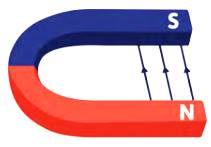
\includegraphics[scale=0.8]{../figs/VN11-PH-25-L-017-1-h92.jpg}
\end{center}
\subsection{Véctơ cảm ứng từ $\vec{B}$}
Véctơ cảm ứng từ $\vec{B}$ đặc trưng cho từ trường về phương diện tác dụng lực. 

Xét trường hợp, một dây dẫn dài $l$ có dòng điện $I$ chạy qua đặt trong từ trường có phương \textbf{vuông góc} với đoạn dây dẫn. Lực từ tác dụng lên dây có độ lớn $F$. Vectơ cảm ứng từ tại vị trí đặt dây có:
\begin{itemize}
	\item điểm đặt: tại điểm ta xét.
	\item hướng: trùng với hướng của từ trường tại điểm đó. 
	\item độ lớn: 
		\begin{equation}
	B=\dfrac{F}{Il},
	\end{equation}
Đơn vị của cảm ứng từ là Tesla (T).	
\end{itemize}
\subsection{Lực từ $\vec{F}$ tác dụng lên dây dẫn mang dòng điện}

\begin{itemize}
	\item Điểm đặt: đặt tại trung điểm của đoạn dây.
	\item Phương: vuông góc với mặt phẳng chứa dây dẫn và đường cảm ứng từ.
	\item Chiều: xác định theo quy tắc bàn tay trái.  
	
	\begin{center}
		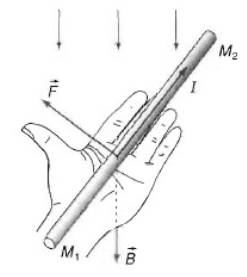
\includegraphics[scale=0.8]{../figs/VN11-PH-25-L-017-1-h105.jpg}
	\end{center}
\textbf{Quy tắc bàn tay trái:} Đặt bàn tay trái sao cho các đường sức từ hướng vào lòng bàn tay, chiều từ cổ tay đến ngón tay giữa hướng theo chiều dòng điện thì ngón tay cái choãi ra $90^\circ$ chỉ chiều lực $\vec{F}$ tác dụng lên đoạn dây.	
	
	\item Độ lớn: 
	\begin{equation}
	F=BIl\sin \alpha,
	\end{equation}
	trong đó,
	\begin{itemize}
		\item $B$ là cảm ứng từ.
		\item $I$ là cường độ dòng điện qua dây dẫn.  
		\item $l$ là chiều dài của đoạn dây dẫn.
		\item $\alpha$ là góc hợp bởi $\vec{B}$ và $\vec{l}$.
		\item $F$ là lực tác dụng lên dây dẫn. 
	\end{itemize}
	
\end{itemize}	


\section{Bài tập}
\begin{dang}{Công thức tính lực từ tác dụng lên dây dẫn mang dòng điện}
\end{dang}

\textbf{Phương pháp giải}

Áp dụng công thức $	F=BIl\sin \alpha$, từ đó tìm được giá trị lực $F$ tác dụng lên dây dẫn, cảm ứng từ $B$, cường độ dòng điện $I$ qua dây dẫn, chiều dài $l$ của đoạn dây dẫn, góc $\alpha$ hợp bởi $\vec{B}$ và $\vec{l}$.

\vspace{1em}
\viduii{2}{	
Một đoạn dây dẫn thẳng MN dài 6 cm có dòng điện 5 A đặt trong từ trường đều có cảm ứng từ $B=\text{0,5}\ \text{T}$. Lực từ tác dụng lên đoạn dây có độ lớn $F=\text{7,5}\cdot 10^{-2}\  \text{N}$. Tính góc $\alpha$  hợp bởi dây MN và đường cảm ứng từ?
	\begin{mcq}(4)
		\item  $30^\circ$.
		\item  $45^\circ$.
		\item  $60^\circ$.
		\item  $90^\circ$.
	\end{mcq}}
{	
\begin{center}
		\textbf{Hướng dẫn giải:}
\end{center}
	
	Góc $\alpha$ hợp bởi dây MN và đường cảm ứng từ là
	
	$\sin \alpha=\dfrac{F}{BIl}=\dfrac{F}{BIl}=\dfrac{1}{2}$.
	
	$\Rightarrow \alpha=30^\circ$.

\textbf{	Đáp án: A.}
}

\viduii{2}{	
Một đoạn dây dẫn dài 20 cm, có dòng điện $\text{0,5}\ \text{A}$ chạy qua đặt trong từ trường đều có $\text{0,15}\ \text{T}$. Biết đường sức từ vuông góc với dây dẫn và đều nằm trong mặt phẳng ngang. Lực từ tác dụng lên dây có độ lớn và phương như thế nào?
	\begin{mcq}
		\item Lực $\vec{F}$ có phương thẳng đứng, độ lớn  $F=4\cdot 10^{-3}\ \text{N}$.
		\item Lực $\vec{F}$ có phương thẳng đứng, độ lớn  $F=2\cdot 10^{-3}\ \text{N}$.
		\item Lực $\vec{F}$ có phương nằm ngang, độ lớn  $F=2\cdot 10^{-3}\ \text{N}$.
		\item Lực $\vec{F}$ có phương nằm ngang, độ lớn  $F=4\cdot 10^{-3}\ \text{N}$.
	\end{mcq}
	}{
\begin{center}
		\textbf{Hướng dẫn giải:}
\end{center}
	
	Lực từ tác dụng lên đoạn dây là $F=BIl\sin \alpha=2\cdot 10^{-3}\ \text{N}$.
	
	Lực từ có phương vuông góc với mặt phẳng chứa dây dẫn và đường cảm ứng từ nên lực từ có phương thẳng đứng.

	
\textbf{	Đáp án: B.}
	}

\begin{dang}{Xác định phương, chiều lực từ $\vec{F}$ \\ tác dụng lên đoạn dây dẫn mang dòng điện}
\end{dang}
\textbf{Phương pháp giải}

Lực từ $\vec{F}$ tác dụng lên đoạn dây dẫn mang dòng điện có:
\begin{itemize}
	\item Điểm đặt: đặt tại trung điểm của đoạn dây.
	\item Phương: vuông góc với mặt phẳng chứa dây dẫn và đường cảm ứng từ.
	\item Chiều: xác định theo quy tắc bàn tay trái.  
\end{itemize}


\luuy{Khi các đường sức từ song song hoặc trùng với đoạn dây dẫn thì lực từ tác dụng lên đoạn dây dẫn bằng 0 hay $F=0$.}

\viduii{3}{

Trong các hình vẽ sau, hình vẽ nào chỉ đúng chiều lực $\vec{F}$ tác dụng lên đoạn dây?

\begin{mcq}(4)
	\item 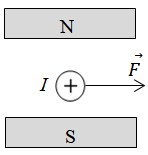
\includegraphics[scale=0.7]{../figs/VN11-PH-25-L-017-1-h93.jpg}
	\item 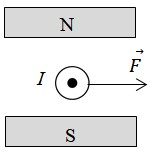
\includegraphics[scale=0.7]{../figs/VN11-PH-25-L-017-1-h94.jpg}
	\item 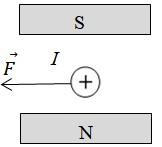
\includegraphics[scale=0.7]{../figs/VN11-PH-25-L-017-1-h95.jpg}
	\item 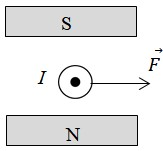
\includegraphics[scale=0.7]{../figs/VN11-PH-25-L-017-1-h96.jpg}
\end{mcq}}{
\begin{center}
	\textbf{Hướng dẫn giải:}
\end{center}

{
	Câu A, D là sai vì theo quy tắc bàn tay trái thì lực $\vec{F}$ tác dụng lên đoạn dây có chiều từ phải sang trái.
	
	Câu C là sai vì theo quy tắc bàn tay trái thì lực $\vec{F}$ tác dụng lên đoạn dây có chiều từ trái sang phải.
	
\textbf{	Đáp án: B}
}
}
\viduii{3}{

Trong các hình vẽ sau, hình vẽ nào chỉ đúng chiều cường độ dòng điện $I$?
\begin{mcq}(4)
	\item 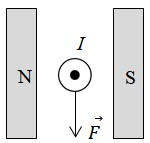
\includegraphics[scale=0.7]{../figs/VN11-PH-25-L-017-1-h97.jpg}
	\item 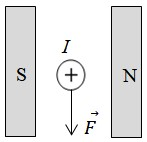
\includegraphics[scale=0.7]{../figs/VN11-PH-25-L-017-1-h98.jpg}
	\item 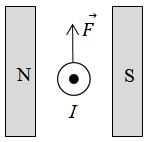
\includegraphics[scale=0.7]{../figs/VN11-PH-25-L-017-1-h99.jpg}
	\item 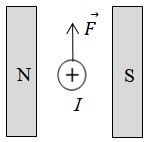
\includegraphics[scale=0.7]{../figs/VN11-PH-25-L-017-1-h100.jpg}
\end{mcq}}{
\begin{center}
	\textbf{Hướng dẫn giải:}
\end{center}

{ Câu A là sai vì theo quy tắc bàn tay trái thì cường độ dòng điện phải hướng từ ngoài vào trong mặt phẳng giấy. 
	
Câu B, D là sai vì theo quy tắc bàn tay trái thì cường độ dòng điện phải hướng từ trong ra ngoài mặt phẳng giấy. 
	
\textbf{	Đáp án: C.}
}

}


